\section*{Classes de Complexité : Le Panthéon }

\subsection*{La Règle d'Or : Pourquoi simplifier $T(n)$ ?}

Le coût théorique $T(n)$ est souvent trop détaillé pour être exploitable (ex: $15n^2 + 7n + 12$ ). En informatique, on cherche surtout à savoir comment l'algorithme se comporte quand $n$ devient \textbf{gigantesque}.

\begin{Comprendre}
 \textbf{La Règle d'Or :} Pour définir la classe de complexité, on ne garde que le \textbf{terme dominant} (celui de plus haut degré) et on supprime tous les coefficients multiplicateurs.
\end{Comprendre}

\textbf{Exemples de simplification (passage au Grand $O$) :}
\begin{itemize}
    \item $T(n) = 2^n + n^{120} \implies O(2^n)$ : Une exponentiation surpasse n'importe quel polynôme.
    \item $T(n) = n^2 + 2n \implies O(n^2)$ : Le $n^2$ « écrase » le $2n$ quand $n$ grandit.
    \item $T(n) = 5n^3 + 10n^2 + 50 \implies O(n^3)$ : On ne garde que la puissance la plus haute.
    \item $T(n) = 100n + 5 \implies O(n)$ : Même avec un gros coefficient, la croissance reste linéaire.
    \item $T(n) = 42 \implies O(1)$ : Un nombre constant ne dépend pas de la taille des données.
\end{itemize}

\subsection*{Le scénario du « Pire des Cas » }

La complexité $O(f(n))$ ne décrit pas une performance moyenne, mais une \textbf{garantie de sécurité}. On calcule toujours le nombre maximum d'opérations nécessaires dans le scénario le plus défavorable.

\textbf{Exemple : Recherche d'un élément dans une liste de taille $n$ }
\begin{itemize}
    \item \textbf{Meilleur cas :} L'élément est à la 1\textsuperscript{re} position $\implies O(1)$.
    \item \textbf{Pire des cas :} L'élément est à la fin ou absent. Il faut parcourir les $n$ éléments $\implies O(n)$.
\end{itemize}

\begin{Definition}[Complexité en NSI]
En Terminale, quand on parle de complexité, on sous-entend toujours la complexité dans le \textbf{pire des cas}. C'est la certitude que l'algorithme ne sera \textbf{jamais plus lent} que ce que prévoit son Grand $O$.
\end{Definition}

\subsection*{Visualisation de la croissance}
\begin{center}
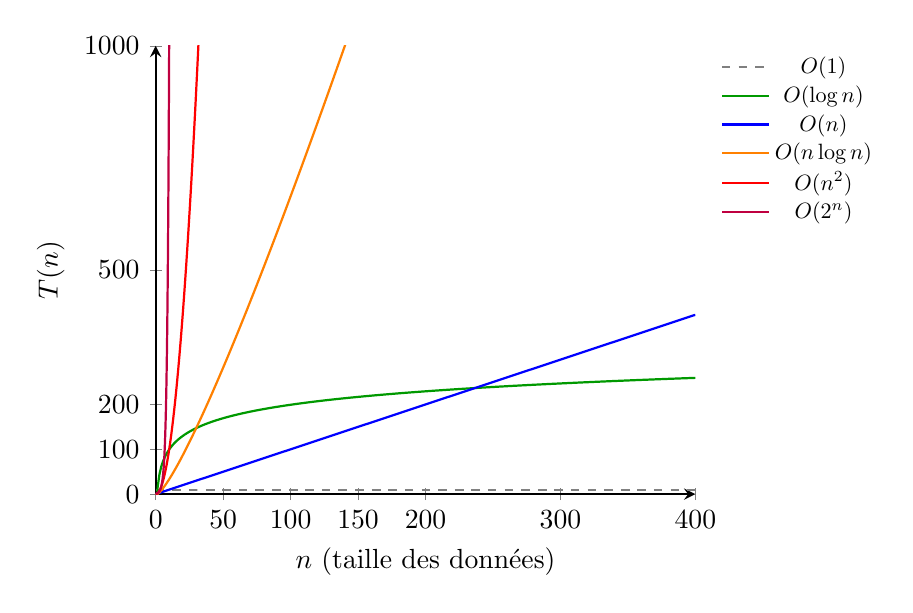
\begin{tikzpicture}[scale=1]
    \begin{axis}[
        axis lines = left,
        xlabel = {$n$ (taille des données)},
        ylabel = {$T(n)$},
        % n s'etend jusqu'a 200
        xmin=0, xmax=400,
        % Le plafond reste a 1000 pour forcer la sortie de cadre
        ymin=0, ymax=1000,
        % Graduation claire
        ytick={0, 100, 200, 500, 1000},
        yticklabels={0, 100, 200, 500, 1000},
        xtick={0, 50, 100, 150, 200, 300, 400},
        % Legende a droite a l'exterieur
        legend pos=outer north east,
        legend style={
            nodes={scale=0.8, transform shape},
            draw=none
        },
        domain=0.1:400,
        samples=300,
        thick,
        no markers
    ]
    % 1. O(1) - Constante
    \addplot [color=gray, dashed] {10}; 
    \addlegendentry{$O(1)$}
    
    % 2. O(log n) - Logarithmique
    \addplot [color=green!60!black] {30 * ln(x)/ln(2)}; 
    \addlegendentry{$O(\log n)$}
    
    % 3. O(n) - Lineaire
    \addplot [color=blue] {x}; 
    \addlegendentry{$O(n)$}
    
    % 4. O(n log n) - Quasi-lineaire
    \addplot [color=orange] {x*ln(x)/ln(2)}; 
    \addlegendentry{$O(n \log n)$}
    
    % 5. O(n^2) - Quadratique
    % Sort du cadre des n=32
    \addplot [color=red, domain=0:32] {x^2}; 
    \addlegendentry{$O(n^2)$}
    
    % 6. O(2^n) - Exponentielle
    % Sort du cadre immediatement (n=10)
    \addplot [color=purple, domain=0:10] {2^x}; 
    \addlegendentry{$O(2^n)$}
    
    \end{axis}
\end{tikzpicture}
\end{center}

\subsection*{Les 6 familles et leur réalité temporelle (pour $10^9$ op/s)}

\begin{itemize}
    \item \textbf{$O(1)$ (Constante) :} Instantané. Accès direct à un élément (ex: \texttt{liste[0]}).
    \item \textbf{$O(\log n)$ (Logarithmique) :} Ultra-efficace. Exemple : recherche dichotomique.
    \item \textbf{$O(n)$ (Linéaire) :} Raisonnable. Exemple : recherche du minimum.
    \item \textbf{$O(n \log n)$ (Quasi-linéaire) :} Très performant. Exemple : Tri Fusion.
    \item \textbf{$O(n^2)$ (Quadratique) :}  Devient lent pour de grands $n$. Exemple : recherche de doublons.
    \item \textbf{$O(2^n)$ (Exponentielle) :} Inutilisable dès $n = 50$ ($2^{50}$ opérations, soit environ 13 jours à $10^9$ op/s).
\end{itemize}

\begin{center}
\renewcommand{\arraystretch}{1.5}
\begin{tabular}{|l|c|c|c|c|}
     \hline
     \textbf{Famille} & \textbf{$n=50$} & \textbf{$n=100$} & \textbf{$n=1\,000$} & \textbf{$n=10^6$ (1M)} \\ \hline
     $O(1)$ & Instantané & Instantané & Instantané & Instantané \\ \hline
     $O(\log n)$ & Infime & Infime & Infime & Infime \\ \hline
     $O(n)$ & Négligeable & Négligeable & Très rapide & 0,001 seconde \\ \hline
     $O(n \log n)$ & Très rapide & Très rapide & Très rapide & 0,02 seconde \\ \hline
     $O(n^2)$ & Rapide & Rapide & 0,001 seconde & \textbf{17 minutes} \\ \hline
     $O(2^n)$ & \textbf{13 jours} & \textbf{Éternité} & \textbf{Éternité} & \textbf{Éternité} \\ \hline
\end{tabular}
\end{center}

% \vspace{0.3cm}

% \begin{tcolorbox}[colback=blue!5!white,colframe=blue!75!black,title= Aide à la lecture des durées]
% Pour bien comprendre les ordres de grandeur :
% \begin{itemize}
%     \item \textbf{Instantané / Infime / Négligeable :} Plus rapide qu'un battement de paupière (moins de 0,1 seconde). L'utilisateur ne s'aperçoit de rien.
%     \item \textbf{0,001 seconde :} C'est une milliseconde. L'ordinateur peut en faire 1000 à la suite en une seule seconde.
%     \item \textbf{17 minutes :} Le temps de prendre une pause café. On commence à sentir que l'algorithme est lourd.
% \end{itemize}
% \end{tcolorbox}

% \begin{Comprendre}
%  \textbf{Le cas du \texttt{while} :} Contrairement au \texttt{for}, son nombre de tours est souvent imprévisible. Si vous oubliez d'incrémenter votre variable de contrôle, la complexité devient théoriquement \textbf{infinie} (boucle infinie). Votre processeur va chauffer pour rien !  
% \end{Comprendre}